\chapter{GeoGPT}
% OR: \chapter{Model}
\label{cha:architecture}

\begin{comment}
Here you will present the architecture or model that you have chosen and which is (or will be) implemented in your work.
Note that putting algorithms in your report is not always desirable, so in certain cases those might be placed in the appendix.
Code is normally to be avoided in the report itself, but may be included in an appendix or submitted as additional documents.
(The actual code must also be submitted together with the final Master's thesis, but as a zip-file.)

Any off-the-shelf tools and methods that you use in your architecture should have been introduced earlier,
tentatively in the Background chapter (or in the Related Work chapter),
so that they can be referenced here by giving backward pointers to the previous text.

Here, or in a separate chapter (or possibly in the Background chapter or in the Experimental Setup),
you should also discuss the data that you use in your experiments (see Chapter~\ref{cha:data}).

Clearly, a figure showing the architecture is a must, such as Figure~\ref{fig:Architecture}.
Describe all parts of such a figure in reasonable detail in the text, possibly with forward pointers to sections where they will be elaborated on (or backward pointers to sections where tools and methods already have been introduced).
Mention work that motivated your architectural choices, parameter settings, etc.
Those choices should then also be discussed and elaborated on in the Discussion chapter.

\begin{figure}[t!]
    \centering
    \missingfigure{Architecture figure to be added}
    \caption{The missing architecture}
    \label{fig:Architecture}
\end{figure}
\end{comment}

\begin{itshape}
    GeoGPT's source code is available in this GitHub-repository: \url{https://github.com/oskarhlm/masters-thesis}.
\end{itshape}

\vspace{12pt}

This chapter will give a detailed description of the inner workings of \textit{GeoGPT}, the thesis' proposed solution to an \acrshort{acr:llm}-based \acrshort{acr:gis}. GeoGPT is a webpage that features a chat interface and a web map. Users can ask questions through the chat interface and receive answers as text and/or geometries in the map. GeoGPT features \textit{three} different agent types: an \textit{\acrshort{acr:ogc} \acrshort{acr:api} Features} agent, a \textit{Python} agent, and an \textit{\acrshort{acr:sql}} agent. Their differences will be explained in this chapter.

\Autosectionref{sec:high-level-application-architecture} will give a high-level overview of GeoGPT's architecture. GeoGPT employs a client-server architecture, where the server is supported by auxiliary services such as databases and external \acrshortpl{acr:api}. The client is a chat-based web \acrshort{acr:gis}, and the server, which hosts the above-mentioned agents, is responsible for streaming responses to the client in the form of chat messages and providing GeoJSON files that can be added to the map on the client. \Autosectionref{sec:agent-architecture} will delve into the architecture of the generic tool agent that is implemented by each of GeoGPT's three agents. This section will also discuss the external tools that the agents have at their disposal, as well as prompt engineering techniques used within GeoGPT.

\section{High-Level Application Architecture}
\label{sec:high-level-application-architecture}

The two main parts of GeoGPT is its web client and its server. They are highlighted in green and blue in \autoref{fig:architecture-overview}, respectively. This is where all of GeoGPT's source code is located. The server is connected to three data sources: a folder containing shapefiles, a PostGIS database, and an \acrshort{acr:ogc} \acrshort{acr:api} Features server. It also uses a Redis database, which is responsible for storing conversations between the user and GeoGPT, and OpenAI's inference \acrshort{acr:api}, which is responsible for text generation. Sections \ref{subsec:langchain-server-architecture} through \ref{subsec:web-ui} will provide further details on the components that make up GeoGPT.

The sequence diagram in \autoref{fig:sequence-diagram} shows how the different parts of the system interact with each other when the user first loads GeoGPT and enters a question into its chat interface. The initial page load triggers the creation of a session object in the Redis database, where the rest of the conversation will be stored. The diagram also illustrates the client-server relationship between the web \acrshort{acr:ui} and the LangChain server. Further details on the sequence diagram will be discussed later in this chapter.

\begin{figure}
    \centering
    \makebox[\textwidth][c]{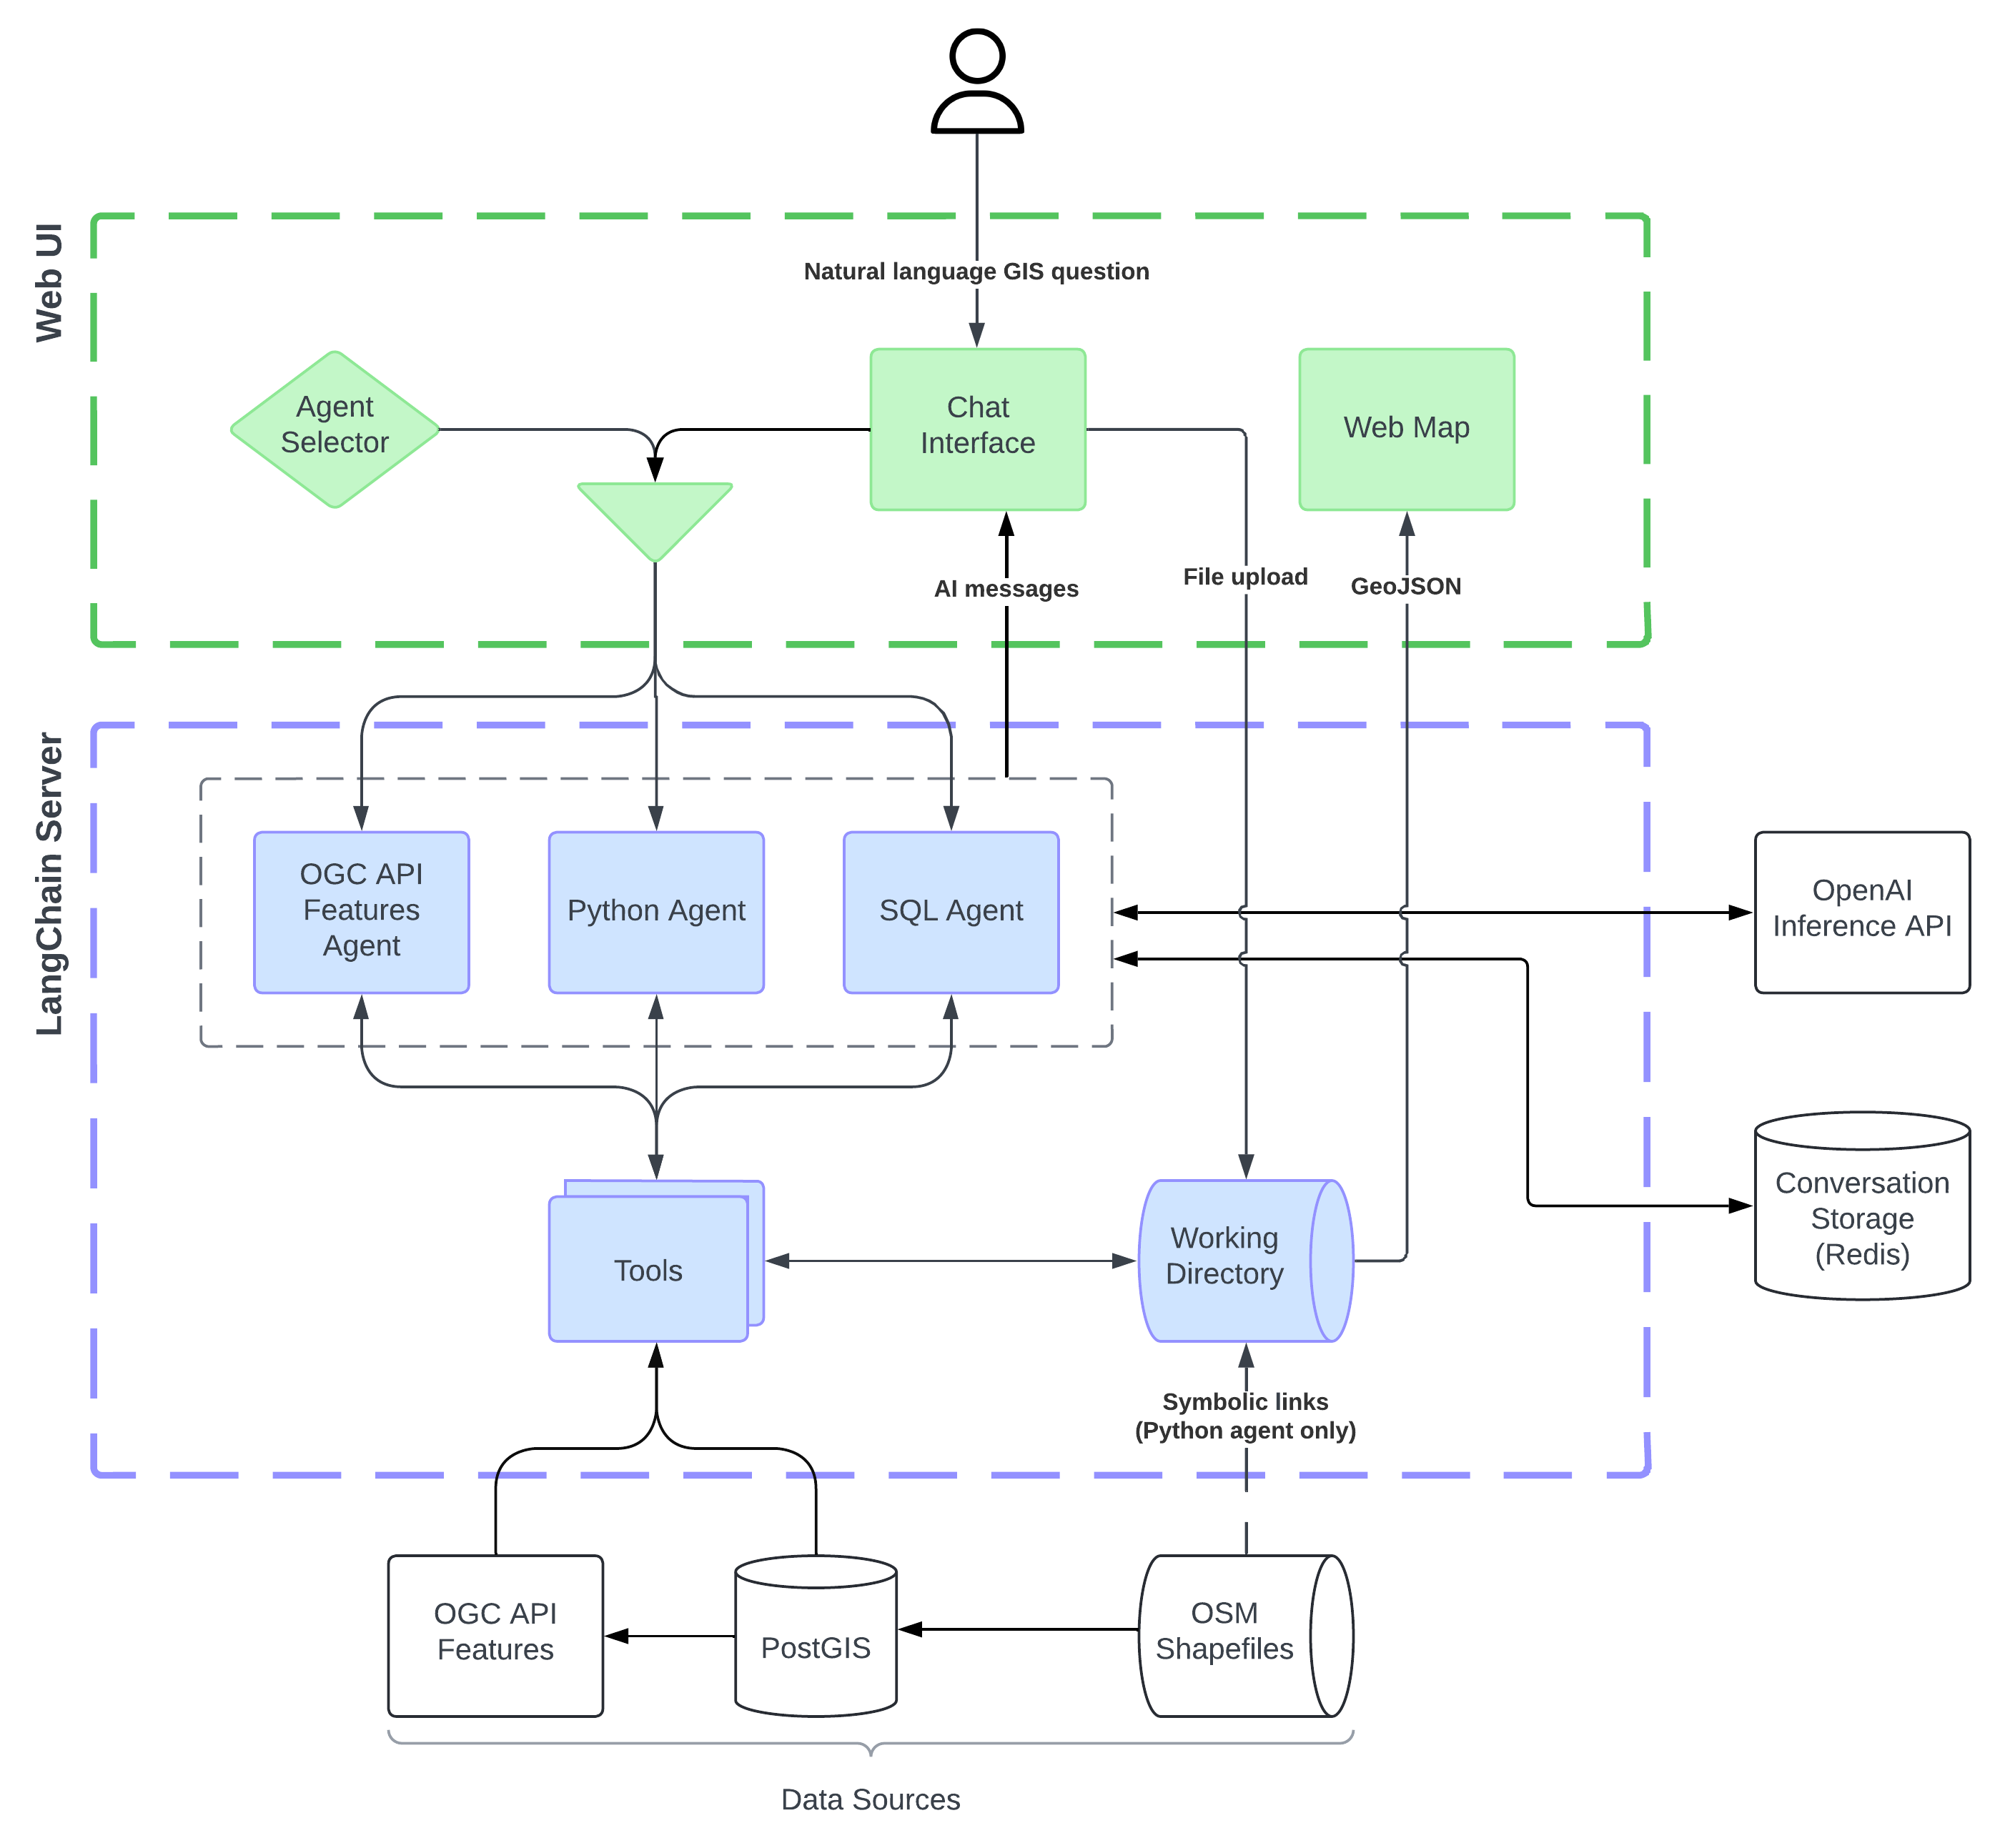
\includegraphics[width=1.2\textwidth]{architecture_overview.png}}
    \caption[Architecture overview for GeoGPT]{Architecture overview highlighting the client-server architecture of GeoGPT, and the major components that make up the Web UI (in green) and the LangChain Server (in blue). Auxiliary services like databases and external \acrshortpl{acr:api} are shown in white.}
    \label{fig:architecture-overview}
\end{figure}

\begin{figure}
    % \centering
    \makebox[\textwidth][c]{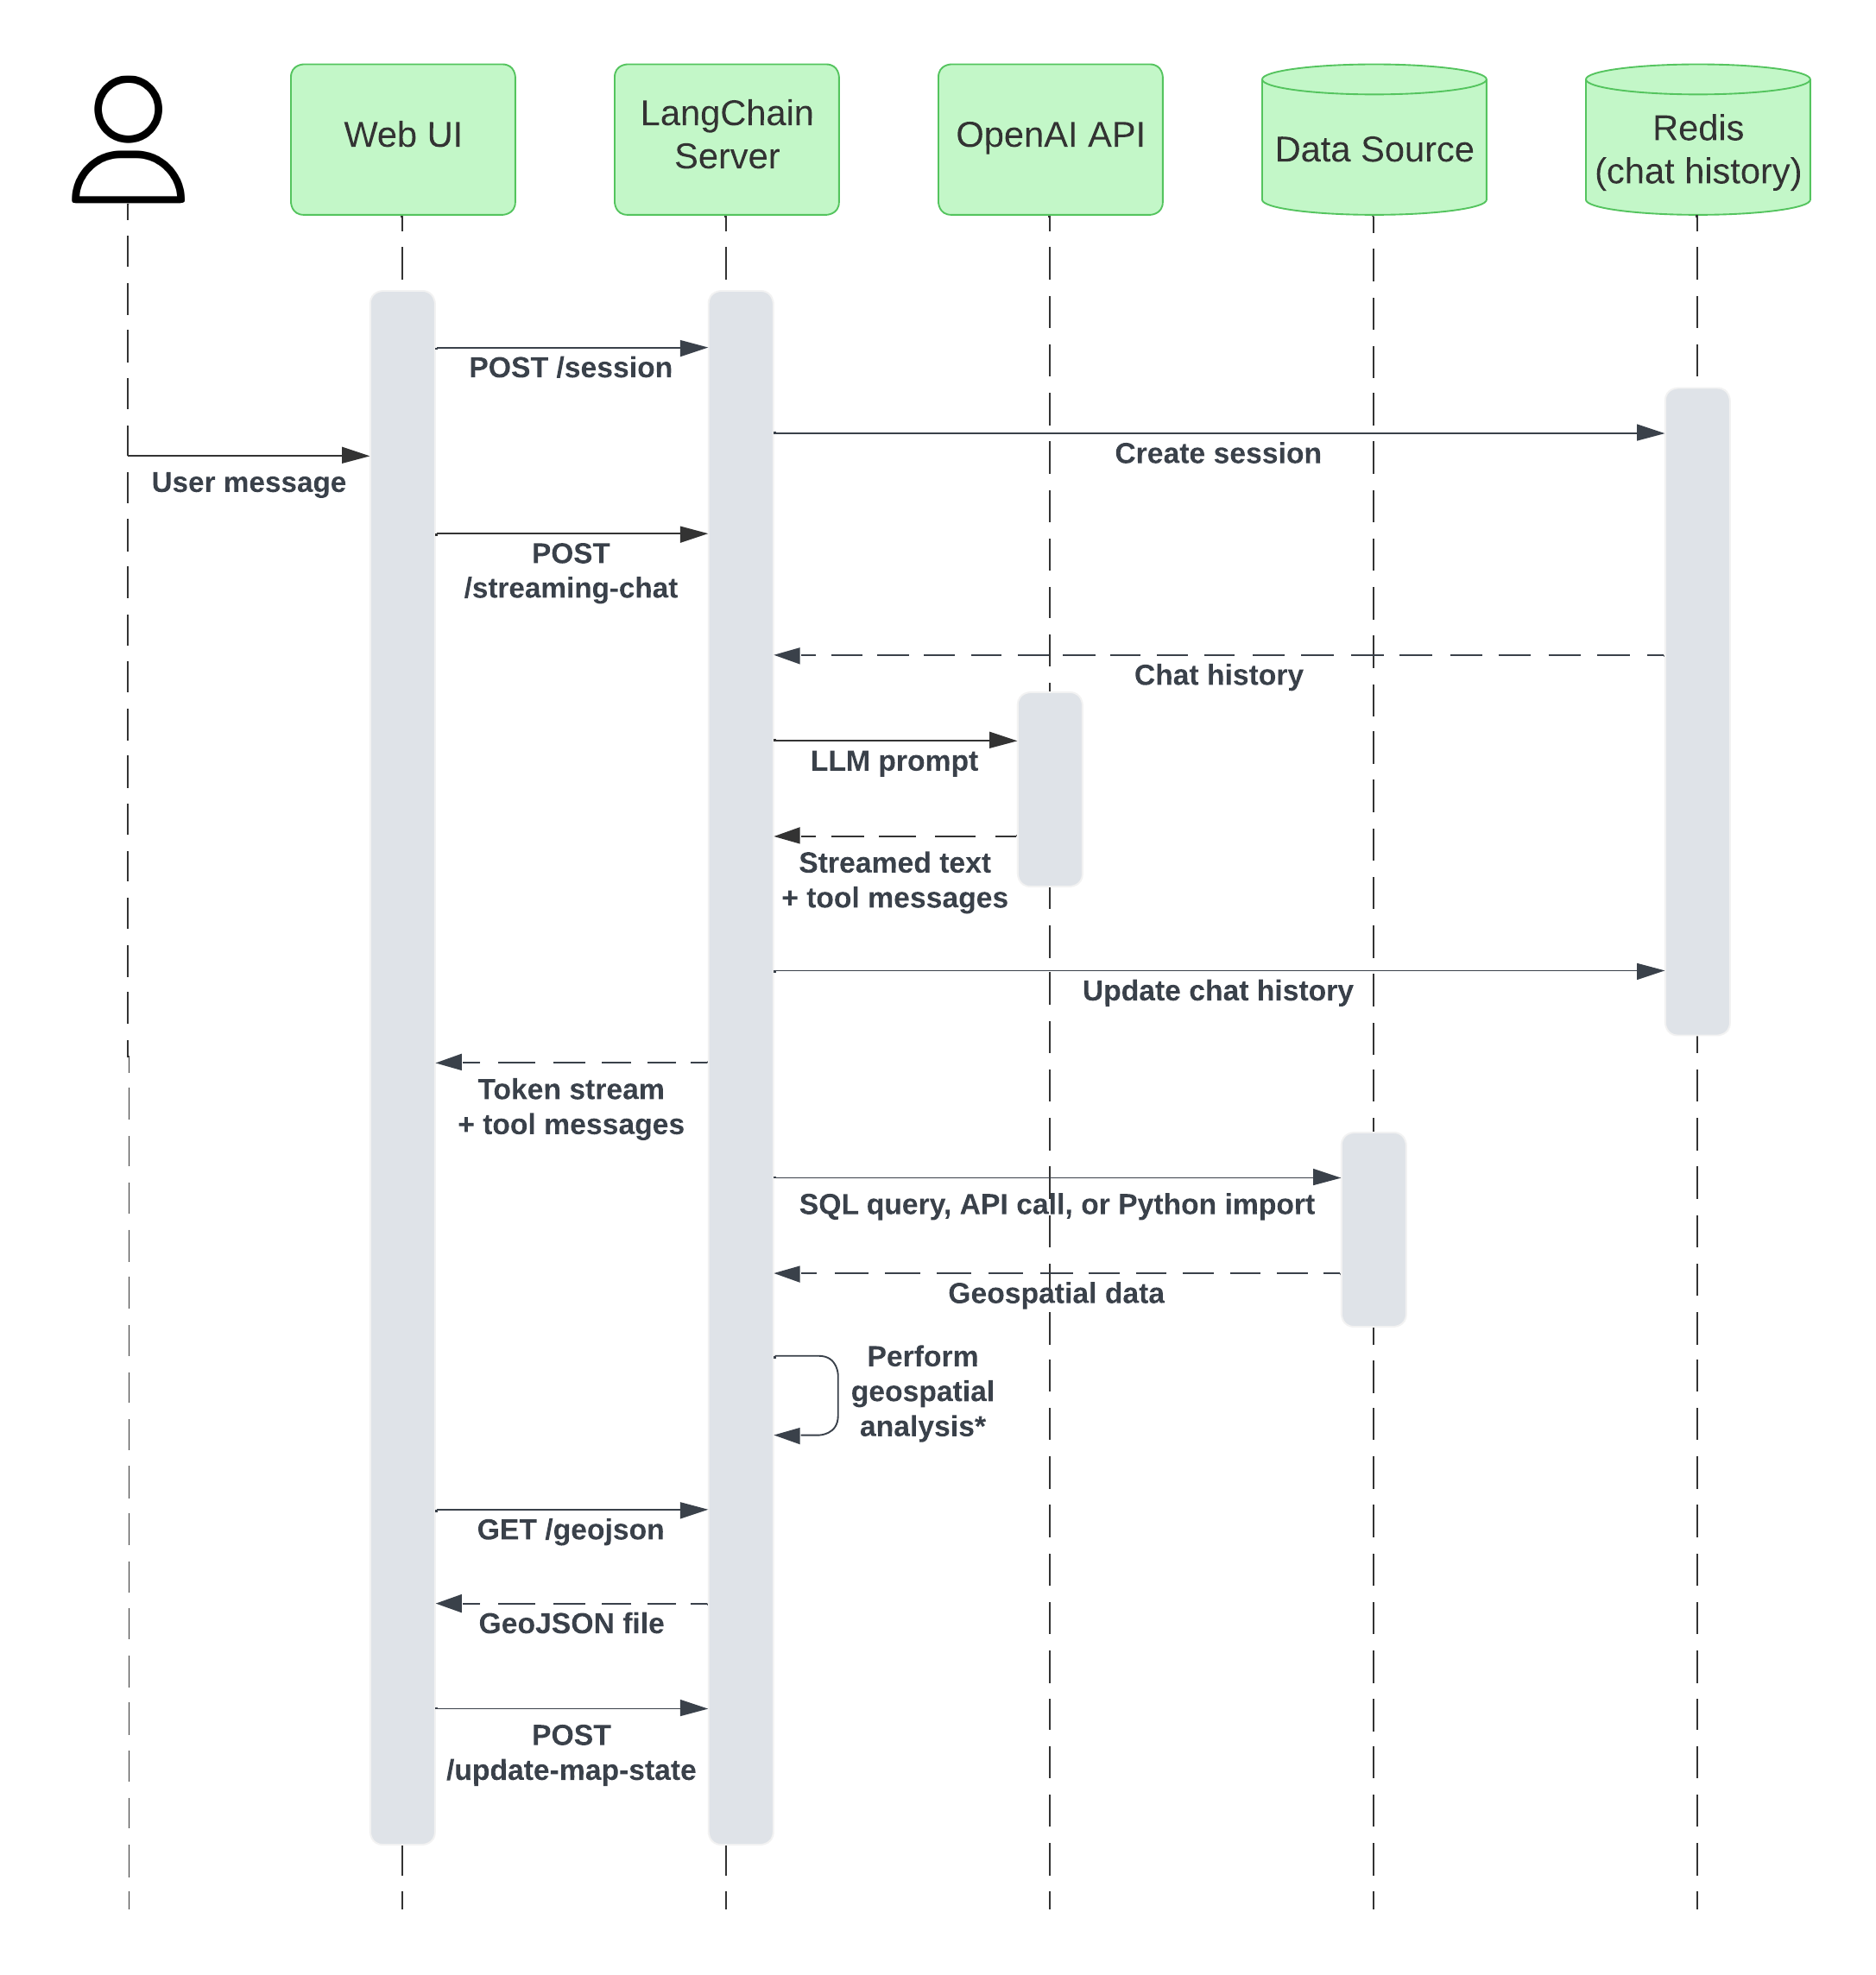
\includegraphics[width=1.2\textwidth]{Sequence diagram.png}}
    \caption[Sequence diagram for GeoGPT]{Sequence diagram showing the information flow as the user sends a message to GeoGPT}
    \label{fig:sequence-diagram}
\end{figure}


\subsection{LangChain Server}\label{subsec:langchain-server}
\label{subsec:langchain-server-architecture}

The \textit{LangChain Server} is the heart of GeoGPT, and is where all the \acrshort{acr:llm}-related logic is situated. It is responsible for taking user messages passed from the web client to the server's \texttt{/streaming-chat} endpoint, and returning a stream of \acrshort{acr:ai} messages generated by an \acrshort{acr:llm}. The \acrshort{acr:ai} messages include textual messages, which are streamed token-by-token, and tool messages, which are discussed in \autoref{sec:agent-architecture}. \autoref{tbl:server-endpoints} shows a complete list of the endpoints exposed by the server, and how they are used by the client.

\begin{table}[H]
    \centering
    \caption[API endpoints exposed by GeoGPT's LangChain server]{Summary of the endpoints exposed by the LangChain server}
    \label{tbl:server-endpoints}
    \begin{tabular}{p{0.22\textwidth}p{0.1\textwidth}p{0.55\textwidth}}
        \toprule
        \textbf{Endpoint} & \textbf{Method} & \textbf{Description}                                                                                                                                                                     \\
        \midrule
        /session          & GET             & Takes a \texttt{session\_id} as a query parameter, allowing the client to continue on a pre-existing session.                                                                            \\
        /session          & POST            & Creates a new session with an empty conversation for a specified agent type.                                                                                                             \\
        /streaming-chat   & GET             & Endpoint for chatting the with the selected GeoGPT agent. Takes a \texttt{message} as a query parameter and returns an event stream, allowing for token streaming from server to client. \\
        /update-map-state & POST            & Used to send the state of the client map to the server. Keeps the server updated on what layers are present in the map, their color, etc.                                                \\
        /geojson          & GET             & Takes a \texttt{geojson\_path} as a query parameter. Allows the client to retrieve a given GeoJSON file that is stored in the working directory on the server.                           \\
        /upload           & POST            & Allows the client to upload one or more files to the working directory on the server.                                                                                                    \\
        \bottomrule
    \end{tabular}
\end{table}

The LangChain server features GeoGPT's three different agent types. These are listed below:

\begin{itemize}
    \item \textbf{\acrshort{acr:ogc} \acrshort{acr:api} Features Agent} -- Retrieves data from an \acrshort{acr:ogc} \acrshort{acr:api} Features server, and uses Python to perform analyses on this data.
    \item \textbf{Python Agent} -- Accesses and manipulates shapefiles using Python code.
    \item \textbf{SQL Agent} -- Interacts with data stored in a PostGIS database.
\end{itemize}

The agents are responsible for taking messages from the users and utilizing the \textit{external tools} available to them through the \acrshort{acr:llm}'s function calling abilities (see \autoref{subsec:function-calling}) to find answers to the users' geospatial questions. The tools available to each of the agents are presented in \autoref{subsec:tools}.

The agents use OpenAI's inference \acrshort{acr:api} to access \acrshortpl{acr:llm} to generate text and function calls. Prompt engineering techniques are used within the agents to produce prompts that can be used as input to these \acrshortpl{acr:llm}. These techniques are described in further detail in \autoref{subsec:prompt-engineering-architecture}.

The agents have access to a working directory where they can store files on-disk. The agents can access the files in the working directory through some of the tools that are presented in \autoref{subsec:tools}, one of which allows the agents to add GeoJSON files stored in the working directory to the map on the web client. The sequence diagram in \autoref{fig:sequence-diagram} shows how the client requests a GeoJSON file using the server's \texttt{/geojson} endpoint, an action triggered by this tool, which is called \texttt{add\_geojson\_to\_map}.


\subsection{Redis for Conversation Storage}
\label{subsec:redis-architecture}

Redis \citep{sanfilippoRedisRealtimeData2009} is a fast in-memory database that is often applied as a caching database that sits on top of some persistent database. It can also be used for vector-based storage, or as a simple NoSQL database. The latter option is the way that it is used in GeoGPT's architecture, and its sole purpose is to store conversations between GeoGPT and its users. Whenever a user starts a conversation with GeoGPT, a session object is created in the Redis database, as the sequence diagram in \autoref{fig:sequence-diagram} shows. This object contains an array that holds all the messages of the conversation. This array is written to every time the human or GeoGPT produces a message.

Storing messages, either in memory as a simple array or in a database like Redis, is crucial to enable multi-message conversations. In order for an \gls{acr:llm} to act as a conversational agent, a chat history needs to be included in the prompt. In the case of GeoGPT, the entire chat history is included. This has the advantage of providing the \gls{acr:llm} with the complete context for the conversation, but the disadvantage of potentially bloating the context window. Furthermore, as the chat becomes longer, each new token will be both more expensive and take longer to get generated. A long chat history could also make the resulting prompt exceed the token limit of the \gls{acr:llm}, meaning that more tokens are passed to the \acrshort{acr:llm} than can fit in its context window. These issues were not considered much for this project.

\subsection[Shapefiles, PostGIS, and OGC API Features]{Shapefiles, PostGIS, and \acrshort{acr:ogc} \acrshort{acr:api} Features}
\label{subsec:postgis-and-oaf-architecture}

18 shapefiles were downloaded into GeoGPT's environment. These are the geospatial data that GeoGPT's agents will have at their disposal when the user asks a \acrshort{acr:gis}-related question. The data are discussed in detail in \autoref{sec:datasets}. For GeoGPT's Python agent, these shapefiles are \enquote{copied} to its working directory using symbolic links.\footnote{\url{https://en.wikipedia.org/wiki/Symbolic_link} (last visited on 2nd June 2024)} This way, the Python agent can access the files in the download directory where the \textit{actual} file is stored, by using the path to a file in the working directory, which \textit{points} to the real file. This makes the startup of GeoGPT much faster, as we avoid copying the actual contents of the files from the download directory to the working directory.

For the \acrshort{acr:sql} agent, a PostGIS database was deployed using Docker, and populated with the shapefiles described above. The files were given spatial indexes to speed up retrieval of features. For the \acrshort{acr:ogc} \acrshort{acr:api} Features agent,  an \acrshort{acr:ogc} \acrshort{acr:api} Features server was added on top of the PostGIS database, as \autoref{fig:architecture-overview} shows. The server was deployed using the \texttt{pramsey/pg\_featureserv} Docker image \citep{crunchydataCrunchyDataPg_featureserv2024}, which requires a connection string to the PostGIS database. Any table in the database which has a geometry column and a specified \gls{acr:crs}, will be exposed on the server. The server offers functionality like bounding box filtering, result limiting, and \acrshort{acr:cql} filtering. These are added as query parameters in the URL used to fetch a collection's items, for instance:

\begin{quote}
    \texttt{.../collections/\{collection\_id\}/items.json?limit=1000\&filter=name IS NOT NULL\&bbox=10.3388,63.3693,10.4590,63.4500}
\end{quote}

In the internals of the server, this URL will be converted to an \acrshort{acr:sql} query that will be run against the database. Results of the query will be returned as GeoJSON. The current implementation of \textit{pg\_featuresserv} only supports a maximum of 10,000 features per request. \autoref{code:cql-to-sql} shows an example of how \acrshort{acr:cql} code is converted into \acrshort{acr:sql} code:

\begin{lstlisting}[
    language=SQL,
    label=code:cql-to-sql,
    caption={[CQL-to-SQL conversion example]Example of how a \acrshort{acr:cql} filter checking if a point at coordinates (0, 0) resides within a feature's geometry, is converted by \textit{pg\_featureserv} to the corresponding \acrshort{acr:sql} code} 
]
\\ CQL code passed through the `filter` query parameter
within(geom, POINT(0 0))

\\ SQL code that will be run agains the database
ST_Within("geom",'SRID=4326;POINT(0 0)'::geometry)
\end{lstlisting}


\subsection[Web UI]{Web \acrshort{acr:ui}}
\label{subsec:web-ui}

\begin{figure}[h]
    \centering
    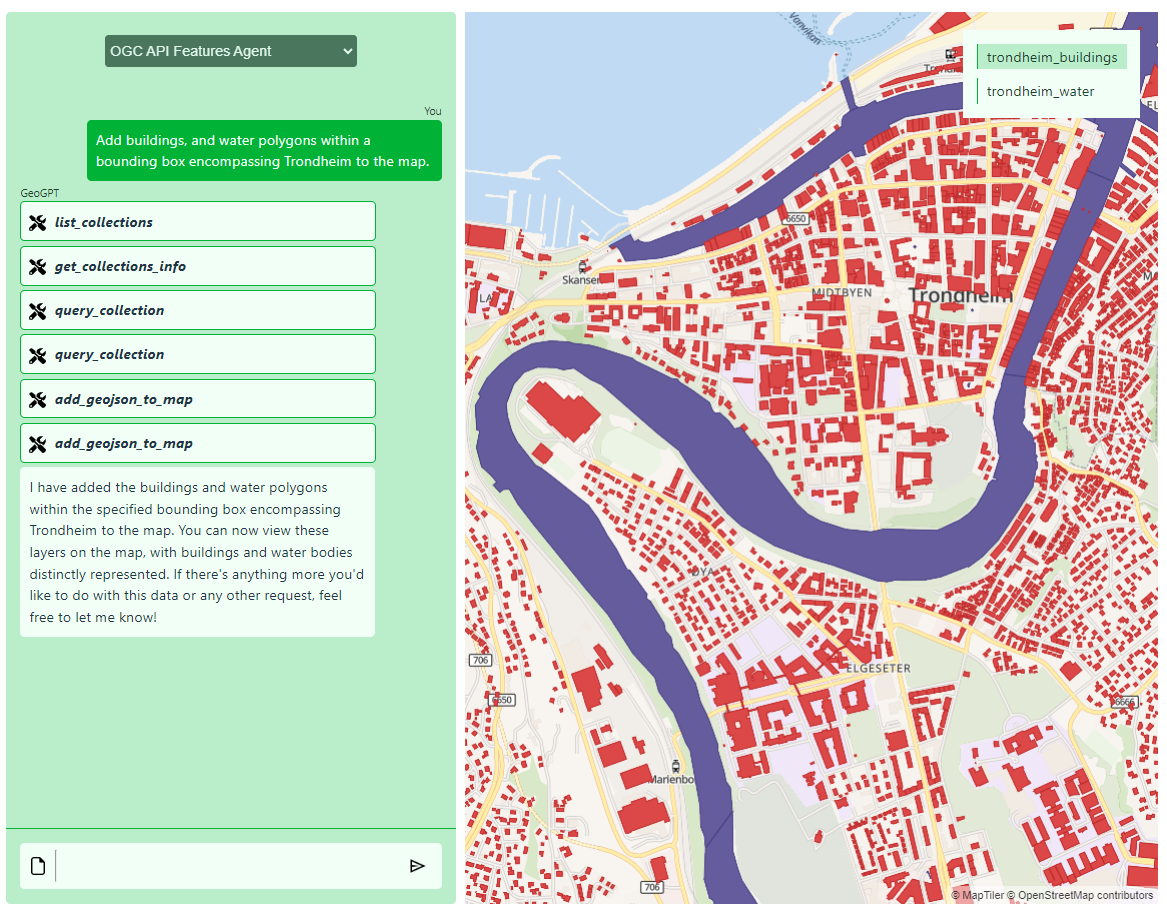
\includegraphics[width=\textwidth]{web_ui_overview_2.png}
    \caption[GeoGPT's web UI]{GeoGPT's web \acrshort{acr:ui}, which features a chat interface and a web map that displays results from analyses. In this example, the user has asked GeoGPT to add water and building geometries for Trondheim to the map. This was successful, as layers named \texttt{trondheim\_water} and \texttt{trondheim\_buildings} were added by GeoGPT, after a series of tool calls.}
    \label{fig:web-ui}
\end{figure}

GeoGPT's user interface is made using SolidJS,\footnote{\url{https://www.solidjs.com/ (last visited on 9th June 2024)}} a JavaScript framework for creating websites. As \autoref{fig:web-ui} shows, it consists of a chat interface, a web map, and an agent selector located above the chat interface. The chat interface was designed to imitate the interface of OpenAI's ChatGPT. In the chat, the user can ask geospatially related questions for GeoGPT to answer. \acrshort{acr:ai} message tokens and tool messages are streamed from the LangChain server and added to the chat, which helps the user follow GeoGPT's thought process as it is solving a problem. The generated text is generally streamed in the Markdown format.\footnote{\url{https://en.wikipedia.org/wiki/Markdown} (last visited on 2nd June 2024)} A library called \textit{showdown}\footnote{\url{https://github.com/showdownjs/showdown} (last visited on 2nd June 2024)} is used to convert the Markdown to \acrshort{acr:html}, ensuring that tables, code blocks, lists, and other elements are properly rendered in the browser. Left of the input field on the bottom of the chat is a file upload button. Files that are uploaded here will be added to the working directory on the LangChain server, as \autoref{fig:architecture-overview} shows.

The map is created using MapLibre,\footnote{\url{https://github.com/maplibre/maplibre-gl-js} (last visited on 2nd June 2024)} an open-source fork of Mapbox.\footnote{\url{https://www.mapbox.com/ (last visited 9th June 2024)}} A base map from \gls{acr:osm} is used, fetched through a mapping platform called MapTiler.\footnote{\url{https://www.maptiler.com/} (last visited on 2nd June 2024)} GeoJSON files that are fetched from the server will be added to the map with a random colour. On the top-right of the map is an overlay listing all layers that are currently present in the map. Using the arrow keys on this list will change the z-index of the selected layer in the map.


\section{Agent Architecture}
\label{sec:agent-architecture}

GeoGPT's agents have a common underlying architecture, which is illustrated in \autoref{subsec:lg-agent-implementation}. They differ, however, through their assigned \textit{tools}, which are described in \autoref{subsec:tools}. Other slight differences are seen in the way that they are prompted. The prompting strategy used for GeoGPT will be discussed in \autoref{subsec:prompt-engineering-architecture}.

\subsection{LangGraph Agent Implementation}
\label{subsec:lg-agent-implementation}

The agentic behaviour of GeoGPT is implemented using LangGraph, which was described in \autoref{sec:langchain}. \autoref{fig:tool-agent-graph} illustrates the flow between the various nodes that make up the agent, and also shows the prompt engineering approach used in GeoGPT. A state dictionary is passed between, and updated by, the nodes. This state includes the chat history, the path to GeoGPT's working directory, a list of the current files in this directory, as well as other less important state.

% The implementation is based upon a prebuilt \texttt{chat\_agent\_executor} implementation from LangGraph.\footnote{\url{https://github.com/langchain-ai/langgraph/blob/main/langgraph/prebuilt/chat_agent_executor.py}}

\begin{figure}
    \centering
    \makebox[\textwidth][c]{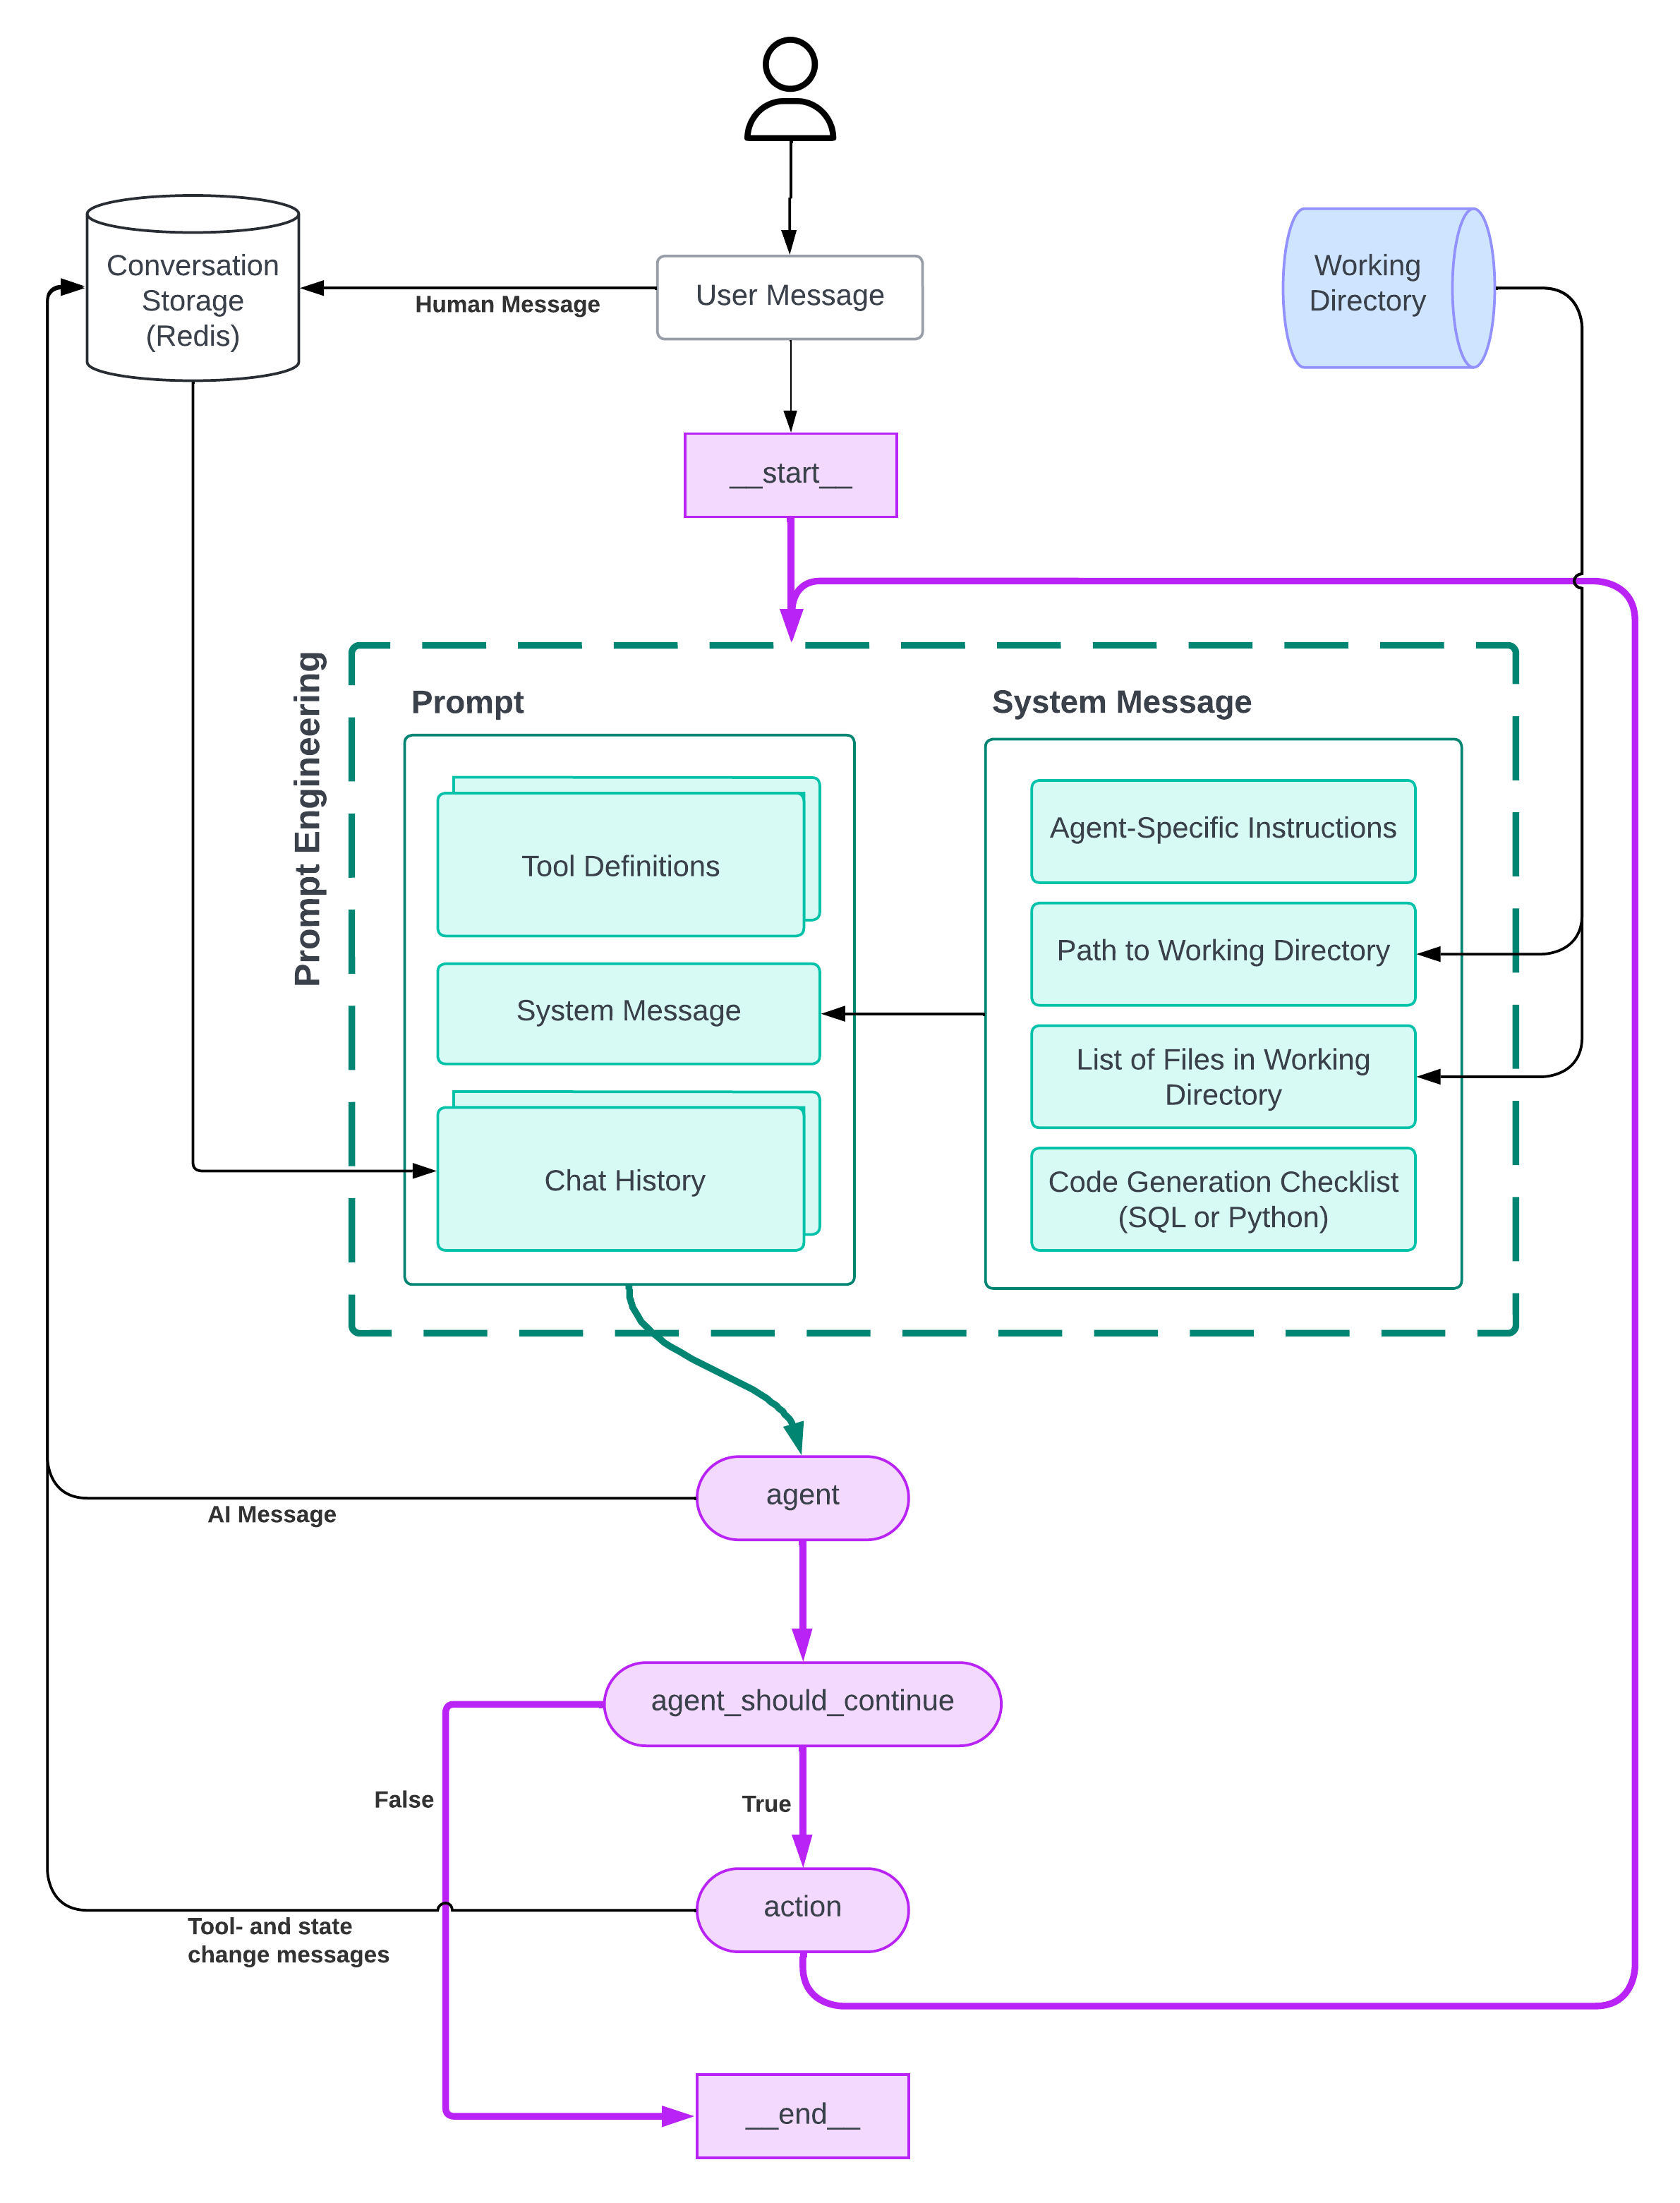
\includegraphics[width=1.0\textwidth]{agent_graph_and_prompt_engineering.png}}
    \caption[Generic tool agent graph including the prompt engineering approach]{Generic tool agent graph including the prompt engineering approach. Purple nodes and edges are what makes up the \textit{LangGraph} graph, while teal-coloured parts are related to prompt engineering.}
    \label{fig:tool-agent-graph}
\end{figure}

The \texttt{\_\_start\_\_} node serves as the entry point of the agent. At this point, only one message is present in the state, namely the initial message from the user. The \texttt{\_\_start\_\_} node points to the \texttt{Prompt Engineering} node, where a prompt is constructed and passed on to the \texttt{agent} node. In the \texttt{agent} node, this prompt is passed to an \acrshort{acr:llm}, so that a response can be generated. This response could contain text and/or instructions to invoke some tool. Therefore, the current state, now containing both the user message and the \acrshort{acr:ai} message, is sent to the conditional node called \texttt{agent\_should\_continue}. This node simply checks if the last \acrshort{acr:ai} message includes instructions to call some tool. If this is the case, we should proceed to the \texttt{action} node.

In the \texttt{action} node, these instructions are used to invoke tools that execute some code. These \acrshort{acr:llm}-generated instructions specify the \textit{name} of the tool, and suitable tool \textit{parameters} that will be passed to this tool (see \autoref{subsec:function-calling} for more details on how \textit{function/tool calling} works). \autoref{code:tool-example-code} shows an example of such a tool. This tool is called \texttt{sql\_db\_query}, and takes a string of \acrshort{acr:sql} code that is executed against a database. After such a tool has been invoked, the return value from the tool is appended as a tool message to the chat history, as \autoref{fig:tool-agent-graph} shows. If the state of the system has now changed because of the tool invocation, a system message is added to the chat history. \autoref{fig:chat-trace-example} illustrates this behaviour, where mid-conversation system messages are added to inform the agent about updates to the state of the system (this further discussed in \autoref{subsec:prompt-engineering-architecture}). We can now loop back to the \texttt{Prompt Engineering} and \texttt{agent} nodes, so that the \acrshort{acr:llm} can react to the results from the tool invocation. This cyclic behaviour allows the agent to repeatedly call tools to try and answer the question from the user. When the agent finds no reason to call any more tools, \texttt{agent\_should\_continue} will return \texttt{False} so that the termination node, \texttt{\_\_end\_\_}, is reached. At this point, the agent has hopefully answered the question from the user.

\begin{lstlisting}[
    language=python,
    label=code:tool-example-code,
    caption={[Tool written in Python that executes SQL code against a PostGIS database]A simplified version of a tool called \texttt{sql\_db\_query}. The tool is written in Python and executes SQL code against a PostGIS database. The \acrshort{acr:llm} will specify the \texttt{query} and \texttt{layer\_name} parameters, both of which are strings. The \texttt{query} will be executed against the PostGIS database, and the results will be saved as GeoJSON under the name \enquote{\{layer\_name\}}.geojson, in GeoGPT's working directory.} 
]
class QuerySQLDataBaseInput(BaseModel):
    query: str = Field(..., description='SQL query to be executed.')
    layer_name: str = Field(
        ..., description='Descriptive name for the data.')


class QuerySQLDataBaseTool(BaseSQLDatabaseTool, BaseTool):
    name: str = "sql_db_query"
    args_schema: Type[BaseModel] = QuerySQLDataBaseInput
    description: str = "Execute SQL queries and manage the results."

    def _run(self, query: str, layer_name: str) -> str:
        try:
            # Execute the query and load the result into a DataFrame
            df = pd.read_sql(query, self.db._engine)

            # Convert WKB to geometries and create a GeoDataFrame
            df['geom'] = df['geom'].apply(
                lambda x: wkb.loads(x, hex=True))
            gdf = gpd.GeoDataFrame(df, geometry='geom')

            # Save the result as GeoJSON
            filename = f'{layer_name}.geojson'
            WorkDirManager.add_file(filename, gdf, save_as_json=True)

            # Return a summary of the SQL query result to the LLM
            return f"Query returned {len(gdf)} features."

        except SQLAlchemyError as e:
            # Inform the LLM of errors in the code
            return f"Error: {str(e)}"
\end{lstlisting}

\begin{figure}
    \centering
    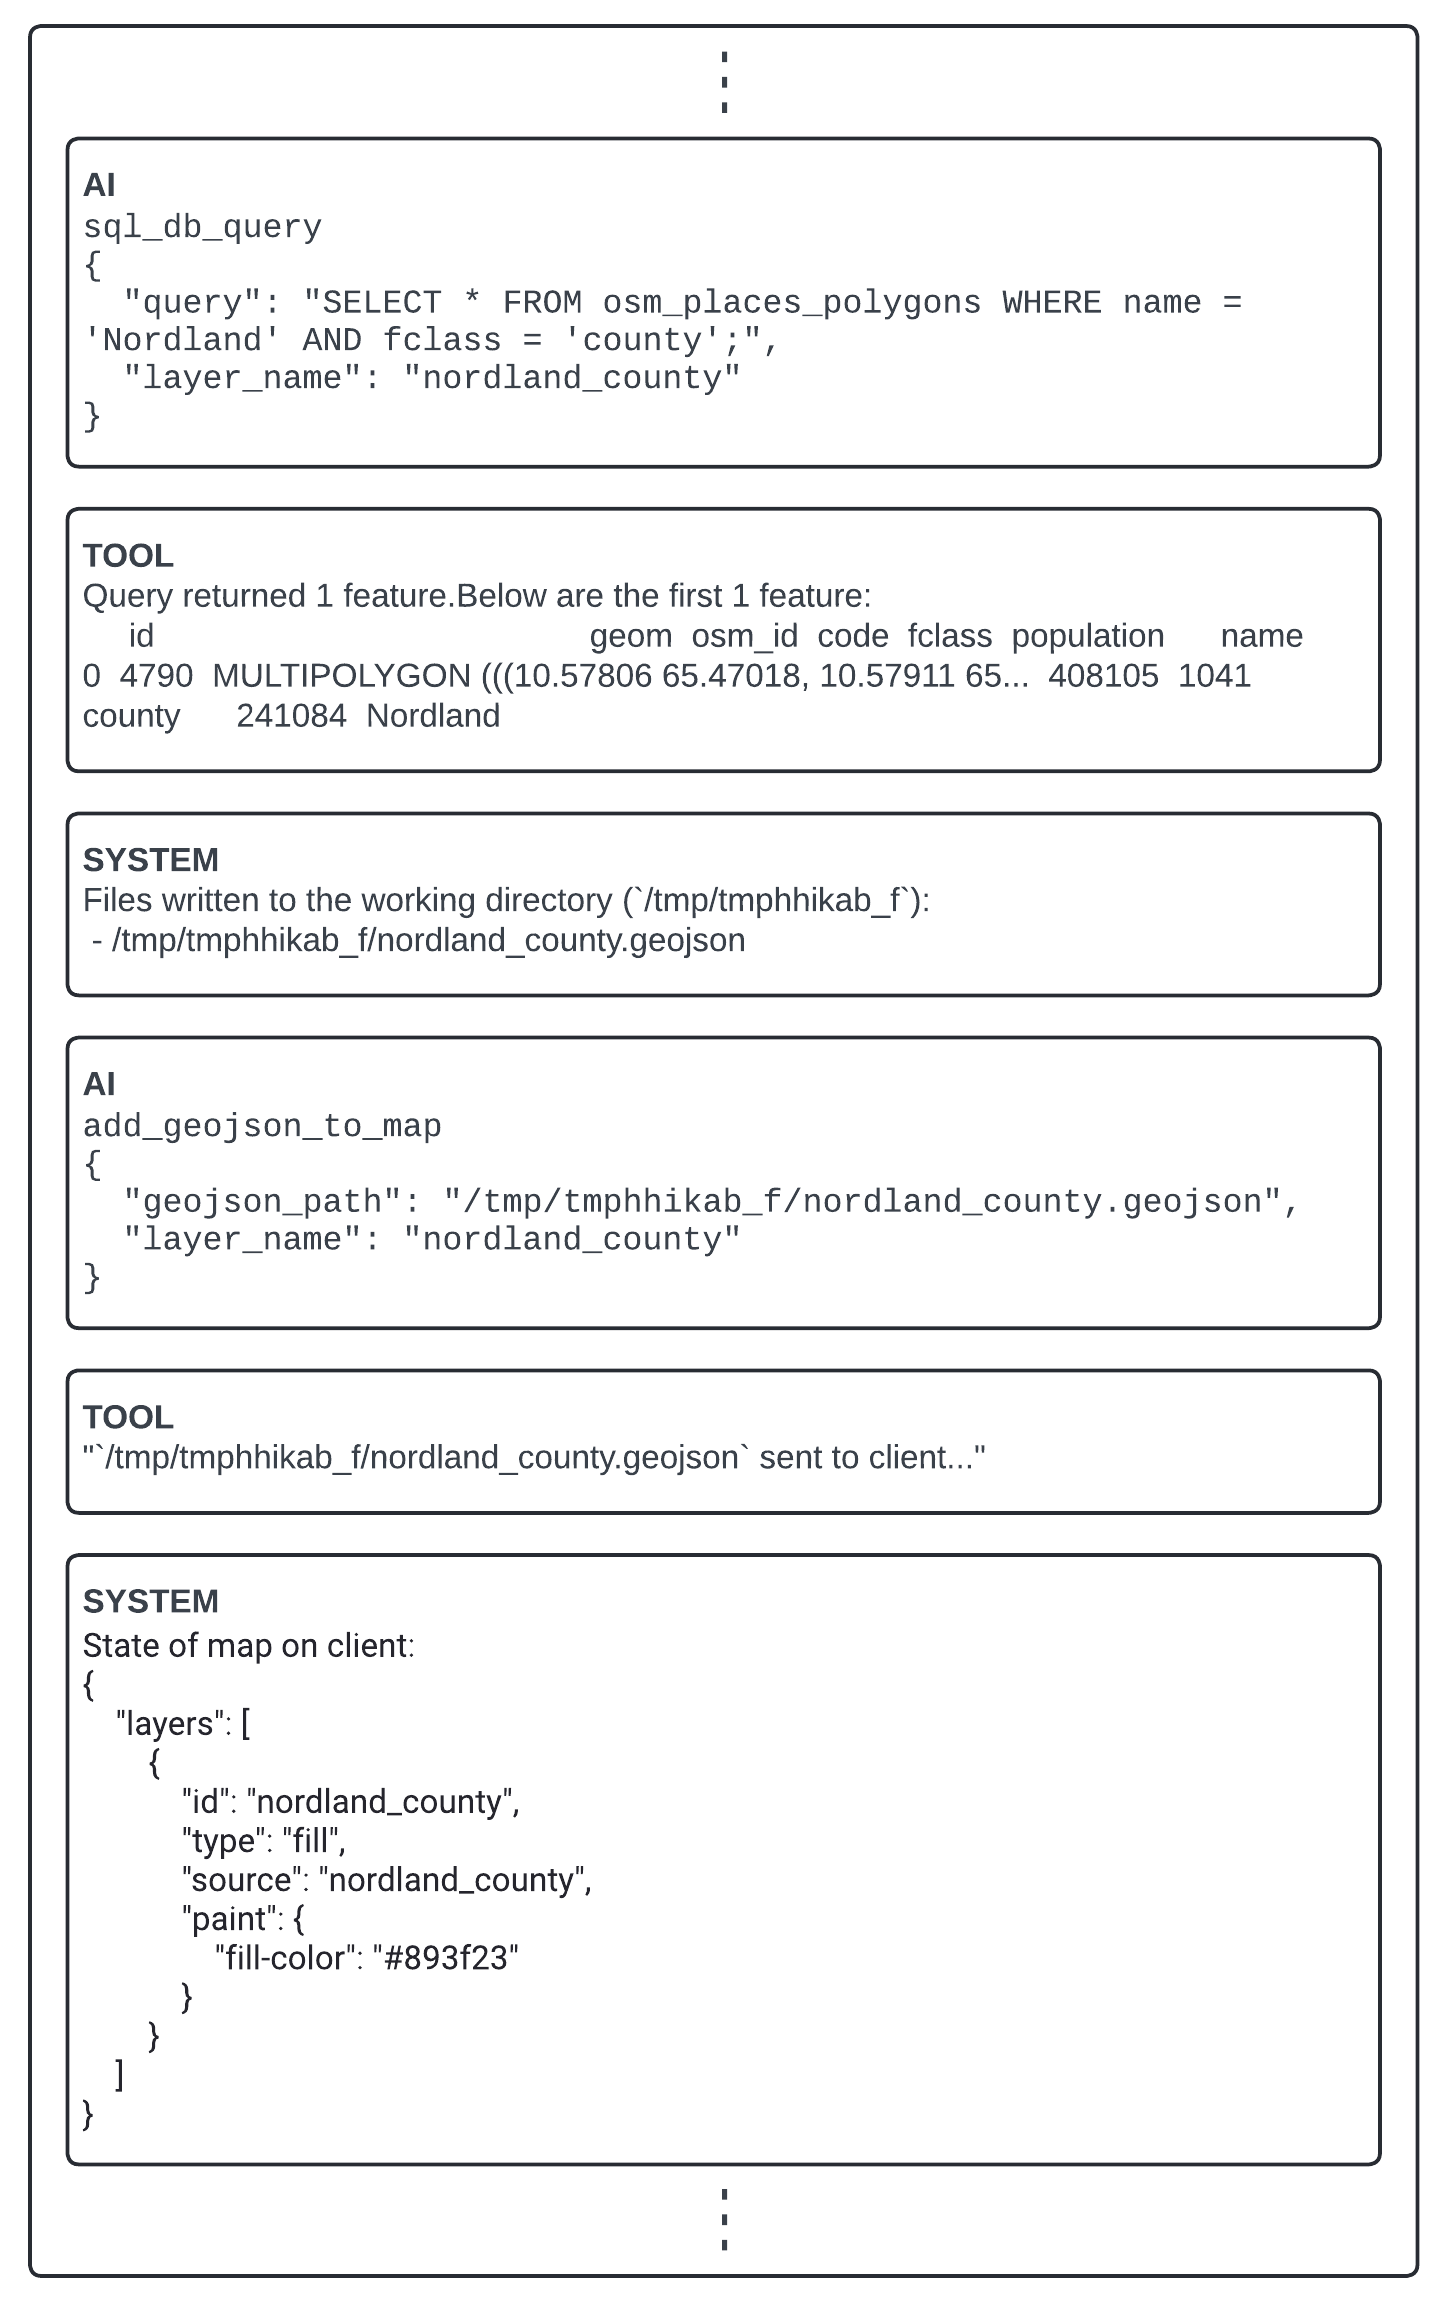
\includegraphics[width=0.8\textwidth]{query_to_client_map_chat.png}
    \caption[Example of a chat history]{Example of a chat history, mid-conversation. GeoGPT elects to invoke the \texttt{sql\_db\_tool} to get a polygon for Nordland county, before adding it to the map using the \texttt{add\_geojson\_to\_map} tool. Tool- and system messages help ensure GeoGPT that the actions it takes are successful.}
    \label{fig:chat-trace-example}
\end{figure}


\subsection{Tools}
\label{subsec:tools}

\begin{table}[h]
    \centering
    \caption{Overview of GeoGPT's agent types and their assigned tools}
    \label{tbl:agent-tool-overview}
    \begin{tabularx}{0.7\textwidth}{XX}
        \toprule
        \textbf{Agent Type}                            & \textbf{Tools}                  \\
        \midrule
        \acrshort{acr:ogc} \acrshort{acr:api} Features & \texttt{list\_collections}      \\
                                                       & \texttt{get\_collections\_info} \\
                                                       & \texttt{query\_collection}      \\
                                                       & \texttt{python\_repl\_ast}      \\
                                                       & \texttt{add\_geojson\_to\_map}  \\
        \midrule
        Python                                         & \texttt{get\_shapefile\_info}   \\
                                                       & \texttt{python\_repl\_ast}      \\
                                                       & \texttt{add\_geojson\_to\_map}  \\
        \midrule
        \acrshort{acr:sql}                             & \texttt{sql\_db\_list\_tables}  \\
                                                       & \texttt{sql\_db\_schema}        \\
                                                       & \texttt{sql\_db\_query}         \\
                                                       & \texttt{add\_geojson\_to\_map}  \\
        \bottomrule
    \end{tabularx}
\end{table}

\autoref{tbl:agent-tool-overview} shows an overview of the tools that are available to each of the agents. As described in \autoref{subsec:function-calling}, these are defined by a name, a description of the tool's functionality, and the parameters that the tool expects. The tools are written by the developer of the system.

% \autoref{code:tool-example-code} shows a tool written in Python that is executes \acrshort{acr:llm}-generated \acrshort{acr:sql} code against a PostGIS database.

The \acrshort{acr:ogc} \acrshort{acr:api} Features agent has access to a total of five tools. \textbf{\texttt{list\_collections}}, which takes no parameters, sends a GET request to the \texttt{/collections} endpoint of the \acrshort{acr:ogc} \acrshort{acr:api} Features server and uses the response to construct a list of the available collections. This tool gives the agent an overview of what collections are available. Using the response from \texttt{list\_collections} the agent can now invoke the \textbf{\texttt{get\_collections\_info}} tool. This tool takes a list of collection names and returns relevant information for each of these collections. This includes the \acrshort{acr:json} response from the \enquote{landing page} of the collection, which includes details such as the collection description, spatial extent, and available attributes. Furthermore, a list of common values for certain high-cardinality attributes is included in the tool's response, as exemplified by \autoref{code:attribute-prevalences}. The percentages for these values are obtained by querying a large number of features from the \texttt{/collections/\{collection\_id\}} endpoint, and calculating the prevalences of the values for these attributes.

\begin{lstlisting}[
    caption={Prevalences of common values for the \textit{fclass} property of the \textit{osm\_natural\_points} collection},
    label=code:attribute-prevalences,
    float, floatplacement=H
]
Property: fclass
    tree: 71.1%
    peak: 27.2%
    beach: 0.9%
    cave_entrance: 0.5%
    spring: 0.2%
    cliff: 0.1%
    volcano: 0.0%
\end{lstlisting}

The \textbf{\texttt{query\_collection}} tool is used to retrieve features from a collection. It takes a collection name, a \acrshort{acr:cql} filter, a bounding box, and a layer name. Based on these parameters, an URL like this is constructed:

\begin{quote}
    \texttt{https://localhost:9001/collections/\{collection\_id\}/items.json?limit=10000\&filter=\{cql\_filter\}\&\{bbox\}}
\end{quote}

The features retrieved from this query are saved in GeoGPT's working directory as \enquote{\{layer\_name\}.geojson}. The message returned from the tool reads something like this: \enquote{Query returned 5627 features.} If the entire GeoJSON response was returned as a tool message, this would quickly bloat the context window of the \acrshort{acr:llm}, and therefore it is avoided.

Common for the \acrshort{acr:ogc} \acrshort{acr:api} Features agent and the Python agent is the \textbf{\texttt{python\_repl\_ast}} tool. This tool takes a string of Python code, executes it, and returns whatever the code prints to the standard output. If the code errors, the error message is returned instead. This Python tool is the main way for these two agents to perform geospatial analyses. The code is executed in a so-called \acrfull{acr:repl}. An advantage of using \acrshortpl{acr:repl} is that code can be executed in blocks, with variables from one block being shared with other blocks. This means that if the first block loads a large file into an in-memory variable, which is often a time-consuming operation, then the subsequent blocks can reuse this in-memory variable without reloading the file. This allows the \acrshort{acr:llm} to quickly retry if the subsequent code blocks should error. The Python agent also has a tool called \textbf{\texttt{get\_shapefile\_info}}, which works similarly to \texttt{get\_collections\_info}.

\textbf{\texttt{add\_geojson\_to\_map}} is the only tool that is common for all three agent types. The tool's job is to add layers to the map on the client. It takes two parameters: the name of a GeoJSON file stored in GeoGPT's working directory, and a layer name. Invoking the tool will send a message to the client, which includes the full path to the file on the server. The client will then make a GET request to the server on the \texttt{/geojson} endpoint, asking for the contents of this file to be returned so that it can be added to the map. The sequence diagram in \autoref{fig:sequence-diagram} illustrates this behaviour.

The \acrshort{acr:sql} agent has tools very similar to the \acrshort{acr:ogc} \acrshort{acr:api} Features agent. \textbf{\texttt{sql\_db\_list\_tables}} is a tool that will list all the available database tables, along with their description. \textbf{\texttt{sql\_db\_schema}} takes a list of table names and returns information about their attributes, the prevalence of different values in high-cardinality columns, and other details about these tables, much like \texttt{get\_collections\_info}. \textbf{\texttt{sql\_db\_query}} accepts arbitrary \acrshort{acr:sql} code that will be executed against the database. \autoref{code:tool-example-code} shows a simplified version of this tool. The tool will make sure that query results that has a geospatial component will be stored as GeoJSON in GeoGPT's working directory, so that the geometries can be added to the map on the client, using the \texttt{add\_geojson\_to\_map} tool.


\subsection{Prompt Engineering}
\label{subsec:prompt-engineering-architecture}

The prompt that is passed to GeoGPT's agents consists of tool definitions, a system message, and a chat history, as \autoref{fig:tool-agent-graph} and \autoref{fig:chat-template} show. It is constructed before every invocation of the \textit{agent} node, where it is passed to an \acrshort{acr:llm} so that it can generate an answer. \acrshortpl{acr:llm} have no inherent memory, so in order to have a chat conversation, the entire chat history needs to be passed with the prompt.\footnote{Several strategies have been developed by researchers to avoid having to pass the entire chat history to the \acrshort{acr:llm} each time, as this will eventually bloat the context window, making token generation slower and worse in quality. Strategies include picking only the $n$ last messages in the chat history, passing a summary of the chat instead of entire messages, and utilizing knowledge graphs.}

\autoref{fig:tool-agent-graph} shows that there are four elements to the main system message:

\begin{enumerate}
    \item Agent-specific instructions
    \item A path to the working directory
    \item A list of the current files in the working directory
    \item A checklist that the \acrshort{acr:llm} should use when generating code
\end{enumerate}

\autoref{fig:chat-template} shows the prompt passed to GeoGPT's \acrshort{acr:sql} agent where the user has asked which county is the largest by size. The agent-specific instructions include information intended to give the \acrshort{acr:llm} contextual awareness and hints on how it should work towards solving tasks. We start by telling \acrshort{acr:llm} that it's a \enquote{helpful \acrshort{acr:gis} agent/consultant that has access to an \acrshort{acr:sql} database containing \acrlong{acr:osm} data}. This is a common way of giving \acrshortpl{acr:llm} a persona, which results in responses like the one in \autoref{fig:effect-of-system-message}. Continuing, we give it some information on how to string tool calls together to solve tasks. We tell it to first list available tables, then look up the schemas of the relevant tables, and then, using the information gathered, to construct an \acrshort{acr:sql} query to answer the user's request. We also remind it that it needs to add the result of the analyses to the map, using the \texttt{add\_geojson\_to\_map} tool.

\begin{figure}[H]
    \centering
    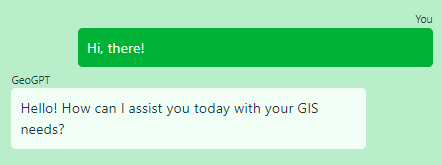
\includegraphics[width=0.6\textwidth]{hi_there.png}
    \caption[LLM persona example]{Conversation showcasing the effect of giving an \acrshort{acr:llm} a persona through the system message}
    \label{fig:effect-of-system-message}
\end{figure}

\begin{figure}
    \centering
    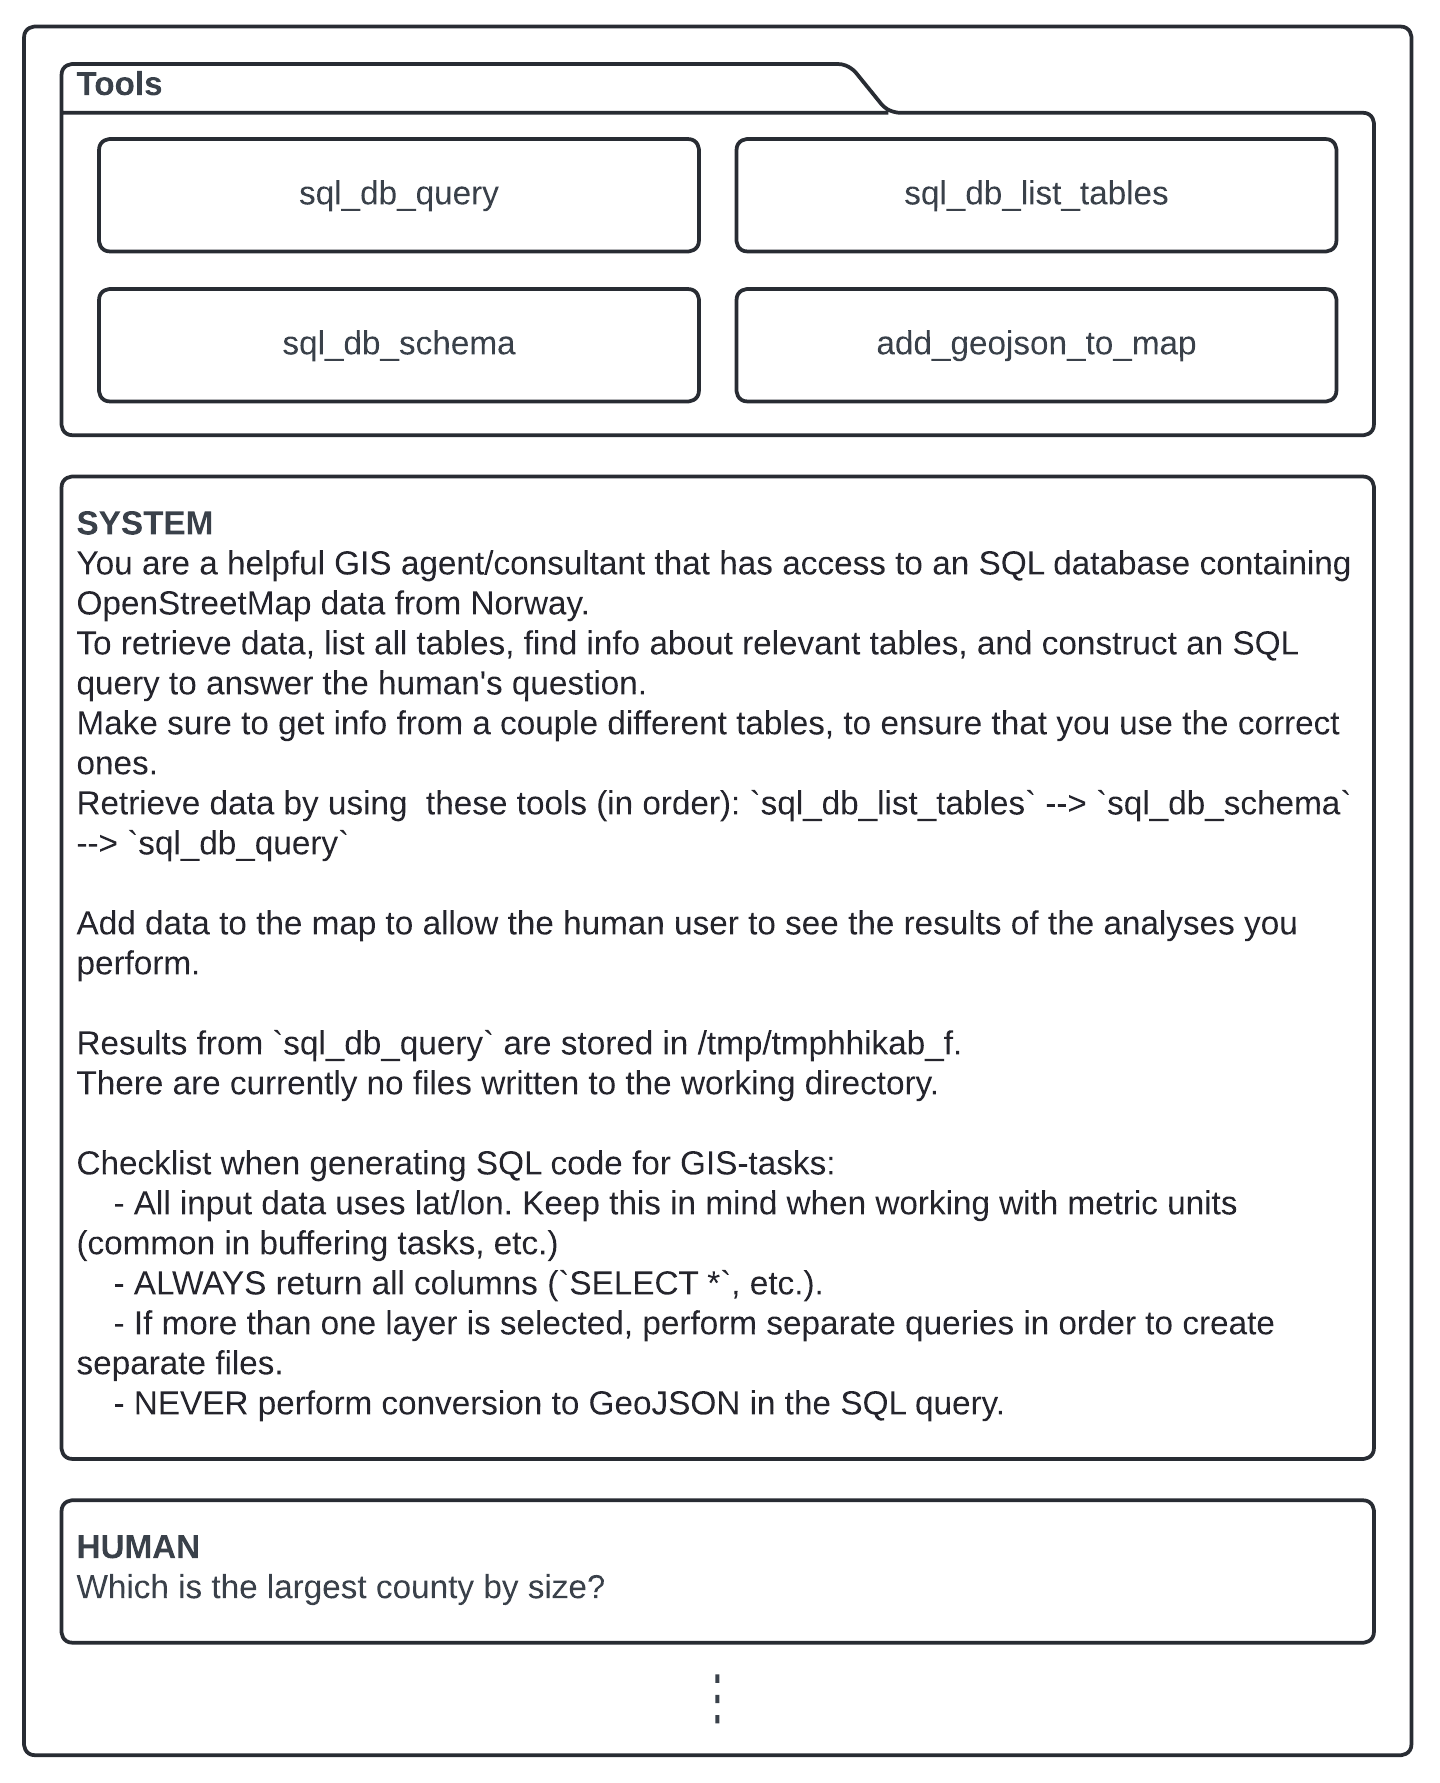
\includegraphics[width=0.9\textwidth]{template.png}
    \caption[Initial prompt to GeoGPT as the user asks a question]{Initial prompt to GeoGPT as the user asks a question. The prompt includes tool definitions, the main system message, and the chat history, which currently only includes the initial message from the user.}
    \label{fig:chat-template}
\end{figure}

The next two parts of the system message concern GeoGPT's working directory. Having a working directory is important to control which files the agent has available, and also to make sure it doesn't save files to the folder on the LangChain server where GeoGPT's source code is located, as this would bloat the actual source code. First, we tell the \acrshort{acr:llm} where the working directory is located. This is especially important for the \acrshort{acr:ogc} \acrshort{acr:api} Features agent and the Python agent, as they need to manually read and write to the paths of the files in the working directory, using the Python code that they generate. Second, we list the files that currently reside in the working directory. In the prompt in \autoref{fig:chat-template} \enquote{There are currently no files written to the working directory}, but if there were any, they would be listed in a bullet point list in place of this message.

The final part of the system message is a checklist to inform the \acrshort{acr:llm} about common pitfalls it could fall into when generating code. The checklist in \autoref{fig:chat-template} is tailored to GeoGPT's \acrshort{acr:sql} agent. A similar checklist for Python is provided for the other two agents, with reminders about using metric \acrshortpl{acr:crs} when doing area calculations, etc.

Normally, conversation-based prompts for \acrshortpl{acr:llm} contain only a single system message, at the very start of the conversation. GeoGPT, however, features a --- to the author's knowledge --- novel usage of system messages. As \autoref{fig:chat-trace-example} shows, system messages are appended mid-conversation, providing updates about state changes in the system. These are generated in the \texttt{action} node (see \autoref{fig:tool-agent-graph}). The first system message is appended because a new file has been added to the working directory, as a result of invoking the \texttt{sql\_db\_query} tool. Such messages help GeoGPT stay up-to-date on what files it has available, and in \autoref{fig:chat-trace-example}, it uses this information immediately to add the new file to the map using the \texttt{add\_geojson\_to\_map} tool. Another system message is eventually appended to tell the GeoGPT that client map has been modified. This message helps ensure GeoGPT that the invocation of \texttt{add\_geojson\_to\_map} was successful. If it wasn't, then the system message would inform it about this.

\glsresetall


